\documentclass[11pt]{article}
\usepackage{amsmath}
\usepackage{graphicx}
\begin{document}
\noindent
\subsection*{Some terms}
Square of L2 $||\theta ||^{2}_{2}$\\
Sum of all squares
\\\\
L2 norm $||\theta ||_{2}$\\
Square root of sum of all squares
\\
\\
Collaborative filtering - collaborative filtering is a method of making automatic predictions (filtering) about the interests of a user by collecting preferences or taste information from many users\\
Assumes that one person has same opinion as the other person
\\\\
Inductive learning Assumption - after seeing many training examples result in high accuracy on unobserved examples\\
Hypothesis approximates well\\
\\
average hypothesis only depends on H, does not always lie in H\\
$H_{2} \subset H_{10}$\\
\\
Target function y = f(x)\\
Unbiased learner cannot generalise \rightarrow\) inductive bias
\\\\
h is +ve when h(x) = 1\\
$\geq_{g}$ more general than	 or equal to\\
h_{j} $\geq_{g}$ h_{k} \equiv \forall x \in X (h_{k}(x) = 1) \rightarrow (h_{j}(x) = 1)\)
\\
Not a total order has there may have the same specificity but different hypothesis (maximally specific h)
\\
\\
Consistency: h is consistent iff h(x) = f(x)\\
 h4(\langle0,1\rangle) = 1 \neq f(\langle0,1\rangle) = 0.\\\\
 \textbf{Proposition 1} \\
\)h is consistent with 𝐃 iff every +ve training instance satisfies h and every
-ve training instance does not satisfy h.\\
 \textbf{Proposition 2} \\
\)If h belongs to H, then it is consistent
\subsection*{Naive Bayes}\\
\subsubsection*{Bayes Rule}\\
There can be relatively lesser occurrences of one class
\\
prior odds / likelihood = posterior odds\\
Bayesian thinking\\
How likely is something not going to work?
\\
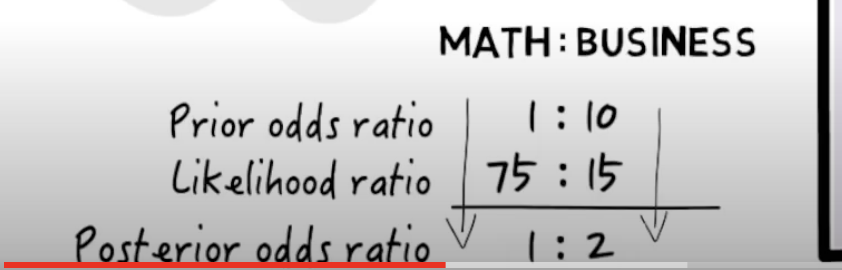
\includegraphics[height=2cm]{images/s4.png}\\
Hold your beliefs, shift your beliefs as u encounter with the world\\
$P(y | x) = \frac{P(x | y) \times P(y)}{P(x)}$
\\
P(X_{1} = 0, X_{2} = -1) = P(X_{1} = 0 \;|\ C_{1}) \times P(X_{2} = -1 \;|\ C_{1}) \times P(C_{1})
+ P(X_{1} = 0 \;|\ C_{2}) \times P(X_{2} = -1 \;|\ C_{2}) \times P(C_{2})
\)
\\\\
\textbf{a priori} - equally probable\\\\\\
Naive - Assuming that features are conditionally independent of each other
\\\\
Insensitive to the number of training examples
\\\\
Calculate which is more likely\\
#1. $P(Outcome | x)$ = P(X_{1} | Outcome) * P(X_{2}| Outcome) * P(Outcome)\\
#2. \)$P(Not\ Outcome | x)$ = P(X_{1}| Not\ Outcome) * P(X_{2}| Not\ Outcome) * P(Not\ Outcome)
\)
\\\\\\
Calculate probability outcome occurs\\
\#1/(\#1+\#2)
\subsection*{Perceptron classifier}\\
x_{0}\theta_{0} + x_{1} \theta_{1} + x_{2}\theta_{2}\\\) of the previous weight vector
\\
first instance will compute based on initial vector\\
For -1, first point checks == -1, != 1 for the points after\\
Update weight = - (x \times\) learning\_rate) for the misclassified instance\\
\\\)
For +1, first point checks != -1, == 1 for the points after\\
Update weight =  + (x \times\) learning\_rate) for the misclassified instance\\
\\
points are linearly separable if there are no longer any misclassified points
not misclassified: sign(x) function having -1 when x is \leq 0
\\\\
\subsection*{Supervised learning}\\
Identifying objects \\
Output would be a continuous value\\
Given many emails, you want to \textbf{determine} if they are Spam or Non-Spam emails.
\\
\\
Given historical weather records, \textbf{predict} if tomorrow's weather will be sunny or rainy.
\\\\
\subsection*{Unsupervised learning}\\
No labels (no output)
Kmeans 
\\
Hard clustering can assign to any one of the cluster\\
\\
Input: Given a set of data points P, number of clusters k
\\1. Randomly pick k points from P as centers $c_{j} = 1.. k$
 \\2.
Iterate (until max-iterations or $c_{j}$ no longer changes up to some threshold) \\
- Assign each point to nearest center: $y_{i}$ = arg min {\parallel p_{i} - c_{j} \parallel}^{2}\)
\\
$c_{j}$ =  Re-estimate each center as mean of points assigned to it
\\\\
Given a set of news articles from many different news websites, find out what are the main topics covered.
\\\\
From the user usage patterns on a website, figure out what different groups of users exist.
\\\\
\subsection*{Motivation}
Importance of models, learning a probability distribution\\
Can learn an arbitrary distribution, not all distribution can be described by the same model\\
Restricted so small number of parameters to be learned in a reasonable amount of time
\\
Can tell water drops and rain\\
Shaking the toy causes the rattling noise\\
Get a good approximation on the cost and structure using limited amount of resources
\\
Data is generated by a physical process\\
\\\\\\
Only wants to capture the signal
\\
Intrinsicity - How many independent dimension are there in each layer\\
\\
\textbf{PCA}\\
z is the reconstruction and v is the principal component\\
Chooses orthonormal bases\\
Ellipse is defined by the eigenvectors and values
\\\\
\textbf{SVD}\\
V - principal components\\\\
$\sum$ - eigenvalues\\
Top left corner will have the largest eigenvalue\\
Bottom right corner have the least significant eigenvalue\\
0 on off-diagonal \\
\\
U - projection of data\\
\\
\textbf{Clustering}\\
k means++ default initialization by sklearn\\
Generalized EM when the approximation is intractable\\
Incremental EM estimates on small number of points, like difference between batch gd and sgd
\\
\subsection*{RL}\\
Key usage: Planning problems, app placements product recommendations\\\\
\textbf{Goal}\\
Low risk when performing actions\\
Goal of markov property: operate in ease\\
choices that maximise the outcome\\
\\
Precision vs control\\
Decisions we make the optimize\\
\\
Prediction allows us to evaluate how good a policy is for a state space\\
Control\\
Reward at any step is optimal, highest reward
\\
continuous MDP - common in robots\\
No supervisor, only reward signal\\
Reward is a scalar feedback\\
whether one state vs the other is preferred\\
\\
RL Challenge: Does not have a good idea if it is right to do, which one is feasible, figuring out rules, which gives the best reward
\\
Given action will give observation and reward\\
Does not know the rules\\
\\
Planning Challenge:\\
A* search - Going through the search space to figure the appropriate action\\
what if i did this, what kind of consequences
\\
Rules are known\\
Uses a search space which requires tree search
\\
\\
Action affects the subsequent states\\
Action $\rightarrow$ Observation (what state it is in) $\rightarrow$  Reward\\
time t will not take the final reward but t - 1\\
Sometimes actions affect the observations\\
May contain irrelevant information of the state at time t\\
Although we have large field of vision, our neural cortex is trying to observe t changes in the environment\\
Function of history is not visible to the environment and is specific to agent\\
State - what information that we have in the brain is what we are going to need to predict the future\\
\\
\textbf{Fully observable}\\
The state can be represented different based on how we want the agent to see the sequence\\
congruent between the agent and the environment\\
\\
\textbf{Partially observable}\\
Align/ localize itself based on the map e.g. game
\\
Represented state can influence the agent
\\
Depending on the agent, we can end up in a different state\\
E.g. if we want to turn the rotor around the corner, it may turn out not to behave that way
\\
Recurrent neural networks\\
Using ReLu to construct each state in deep learning, easy to compute as no exponential operations
\subsubsection*{Policy}
Look through the mapping function\\
Deterministic $s_{1}$ to $a_{1}$ \\
Stochastic Take a particular action with a probability\\
\\
Value function - future reward\\
Sum of expected reward, reward farther in the future will have gamma to discount it\\
Model - probability that it will go to the next state, sum over all possible actions has to be 1
\\\\
\textbf{Agent taxonomy}\\
Value Based\\
Policy - in this state we take a particular action\\
Actor Critic - model based
\\
\subsection*{Exploration vs Exploitation}
Going to the restaurant that i like \\
Exploration - discover more information about the environment
\\
Exploitation - Exploits known information to maximise reward
\\\\
\subsection*{State transition probability matrix}\\
Represented with the symbol P\\
some of the values are 0 in the transition matrix if it cannot move to a particular state\\
episodes are finite\\
there are always probability attach to the state, eventually it will reach the terminal state
\subsection{Markov Reward process}
Attach the reward and discount\\
Differentiating reward,create two different states with different reward\\
$E(r_{t+1} | ..)$ immediately receive the reward in next time step
\\\\
Discount factor$\gamma $
\\ Near sighted - given where i am now where should I go
\\ Far sighted - sum all the rewards add all of them, favor longer samples (should have more reward)
\\
\textbf{Role of Discount}\\
Infinitely sample the cycle, a lot of uncertainties on the future
\subsection{Bellman equation}
Reward based on executing the state
\subsection*{Value iteration}\\
Idea of value iteration\\
Instead of looking what policy to take, look back and determine what is the best action brought us to get the best value function \\\\
Emits the observation and reward\\
Recover information or t and r\\
\\
Value iteration is a simple form of policy iteration\\
Use optimal V*  to create back the policy\\
\subsection*{Q learning}
Use q value to engineer the policy (monodically increasing)\\
r(s, a) reward at comes at next state\\
Higher value of q means we see it a lot of times, smooth it over time
\newpage\noindent
\subsection*{Neural Networks}
$\Theta$ dimension = ($d_{l-1}$ + 1) \times $d_{l}$ where l is the layer before the activation function (denote by x or a)\\
g function will be relu for deep learning and tanh for NN\\
For the hard threshold, when it is close to 0 it becomes a linear line\\
a = g(s) = $g\big(\sum\limits_{j=0}^{d[l-1]} \Theta_{i,j}^{[l]}\ x_{j}^{[l-1]}\big)$
\\
1 represent correct classification
\\
-1 to 1 step function \\ 
Going from -1 to 1
h = \begin{matrix}
[1;-1;-1]
\end{matrix}
where 1 represents the output unit to be positive (for eg first from the top $a_{1}^{[l]}$)
\\\\
Number of kernels N = 2 for gray, 6 for RGB\\
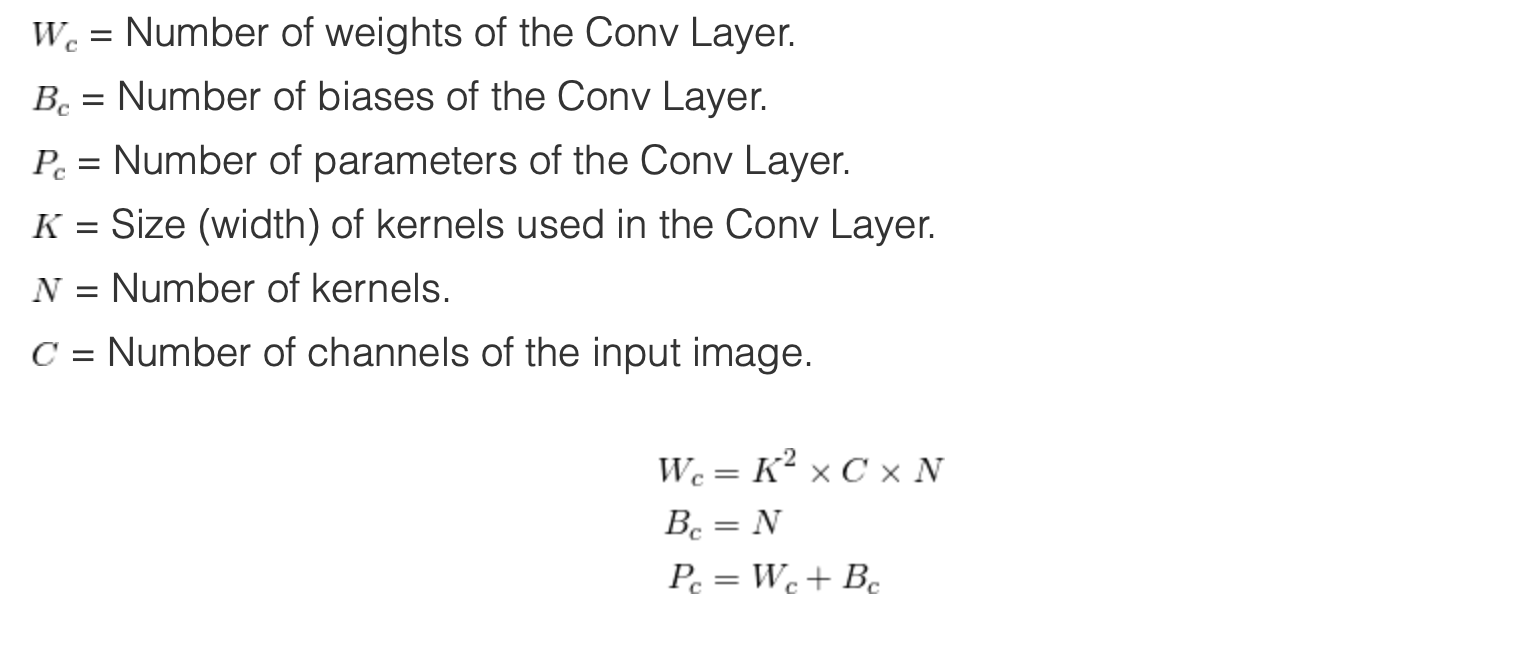
\includegraphics[height=4cm]{images/s6}
\\
\textbf{Motivation}\\
In traditional ml, it is difficult to handcraft features, neural networks are good in feature learning\\\\
NN generalise badly\\
As the number of parameters (weights and layers) increase in a neural network, it can easily overfit the data.\\
Backpropogation is a complicated and tedious process. Moreover, the surface plotted by the error of a neural network in non-convex and high-dimensional and can consist of many hills and valleys - making it hard to reach the optimal set of weights.\\
\\
Do all the neurons in a layer always share the same bias value?
\\
Yes, that is correct.  The bias value is the same value ($x_0=1$) for all units at all layers, because we are going to learn the particular weight for the bias for each individual unit, $\theta_{0}$, separately.  It's just pictorially cleaner to think that each layer has a separate bias unit, but it doesn't matter, because the value of the bias unit is always (by convention) set to unity, such that the individual weights $\theta_{0}$ (or in the NN matrix notation  $\theta^{(l)}_0$ are the controls for the biases. \\\\
\\
Random initialisation of weights for sign function\\
the sign() function takes different constant values in different regions and therefore has gradient 0.\\
the sign() function is discontinuous at x=0.\\
\\
Stack in together in a linear unit\\
Generalise things that are out of sample\\
\\
Regularisation for NN\\
Weight decay square of the weights are small so it is more toward linear regression (L2 regularisation) \\
\\
\\
\\
Is the Soft Weight Elimination function a Cost Function?\\
No, but it closely related.  It is a regulariser, a separate, artificial part of the augmented loss function, as what we learned in Week 05.  We denote regulariser functions as $\Omega(\theta)$.
\\\\
Would it have been a good idea to stop the first time the validation error goes up?\\
The validation error might fluctuate and therefore stopping it the first time it goes up will not give the optimal result. One can consider using a moving average or some other metric.\\
\subsection*{Deep Learning}
Capability to take in multiple input and give multiple outputs\\\\
Dropout - Generalise well rather than approximate well and overfit
ReLU - Vanishing gradients
\\
Bias- Variance tradeoff - Not generalizing due to too many parameters, model representation fit the particularities. Not fitting the additional noise.
\\
\\
Higher budget will have a wide set of solution and encompasses $\theta_{lin}$ (the ideal solution) such that no regularisation is used
\\
$\theta_{reg}$ is proportional to the size of the circle, larger C causes smaller regularisation, smaller circle leads to larger gradient
\\\\
GAN create adversary to help u train better\\
E.g. mock test paper to do better in exam
\\
RNN time series inputs are correlated to each other\\
E.g. determiner followed by noun
\\
Weights of output from one node to another model layer of another time step is the same \\
\\
Model constraint input uses the same weights so that we can fewer parameters than 2
\\
\\
1 to Many: Image captioning\\
Many to 1: Sentiment Classification\\
Many to Many: NMachine translation
Many to Many (time sensitive): Stock market prediction\\
\\
\subsection*{RNN}
Tries to get the softmax chance higher\\\\
\textbf{Truncated backprop}\\
Instead of going to the start, backprop only to the start of the partition block
\subsection*{CNN}
Finding context where locality is important or somehow related to the things nearby\\
Key idea: Make it invariant to position\\
E.g. Non-linear transformation to find a horizontal lines\\
AND and OR gate to form a high level representation\\
\\
Image that maximises the strength of the corresponding units activation\\
\\
Tied samples over all the subsamples of the image\\
Sliding windows to build new feature maps\\
Sub-sampling (Pooling layers)\\
Stride - ignore intermediate squares
Max pooling gives the maximum of the units based on the filter size\\
\\
Layers at the beginning of the network has smaller activations as it is the problem of vanishing gradients (gradient is very small at end layers) stacking all of the layers together, when run on training (after pre-training)
\\
Layers get more positive or negative further down the network as compounding signals get more extreme, causing vanishing problem, doesn't give the same magnitude of gradient at different parts of the network
\\
- Learning rate has to compensate\\
- Weight decay regularisation 
\\\\ 
Or when values are close to 1, then we have issues with learning
\\
ReLu loses representation \\
\\
softmax cannot be used in nlp to predict next word as it can be computationally expensive
\\
hierarchical softmax can be computed in parallel
For unsupervised pre-training, weights by supervised learning and fine tuning it
\\
Final softmax layer needs supervision so we can only pre-train the middle layers
\\
GPU allows operation to happen simultaneously\\
each part of the GPU computing one feature map
\\
\\
performance will only get better for resnet with more layers as the residual will be learned by the next layer only if in the previous layer the residual is not captured.
\subsection*{Sparse Autoencoders}
Have to learn a smaller set of weights like a lossy compression algorithm \\
L1 to encourage sparsity
\subsection*{Dropout}
Idea: Random forest feature projection\\
Keep input fixed and only the output at other layers change\\
Rotate over multiple batches\\
Only certain neuron get the weight which can help in regularisation
\subsection*{Transfer learning}
Unsupervised feature extraction layers, or bottom and middle layers to use for new tasks\\
Hyperparameter to decide where to cut off softmax, FC, pooling
\\
Not useful for\\
VGG net has learned color or natural images that are not part of the domain
\subsection*{Representation Learning}
Uses embedding in the compressed layers
\subsection*{SVM}
Another linear unit
\newpage\noindent
\subsection*{Find S}
1.Initialise h to most specific h\\
2. If the positive instance differs, then replace with ?
\subsection*{Version space}
List all hypothesis, remove any hypothesis that is inconsistent with any training example h(x) $\neq$ f(x)
\subsection*{Candidate Elimination}
prefers positive examples over negatives as there can only be one maximally specific hypothesis in each iteration
? don't care\\
\empty no value\\
Set $S_{0}$ = \langle \emptyset \emptyset \emptyset \emptyset \emptyset \emptyset \rangle\\
\\
$G_{0}, G_{1}$ = \langle ? ? ? ? ? ? \rangle\\
\\
\)
For the negative example,\\
Create h from the specific hypothesis when it differs based on previous instance\\
Remove those that are inconsistent from the previous general hypotheses\\
Keep S to the previous instance S
\\\\
For the positive example,\\
replace with ? when it differs
\\
\subsection*{Cost functions}
Logistic regression\\
Is binary classification\\
Need meta strategies for multi class and it chooses the model that has the highest confidence in predictions
\\
Only gives values 0 and 1 so it is not a good result
\\\\
J(\theta) = \frac{1}{m} \sum\limits_{j = 1}^{m} ln(1 + exp^{-y^{{j}\theta^{T}x^{j}}})\\
\\\)\)
Linear regression\\
J(\theta) = \frac{1}{m} \sum\limits_{j = 1}^{m} (\theta^{T}x^{j} - y^{j})^2

\subsection*{Linear algebra}
trace(AB) = trace(BA) = trace(I_{n+1}) = n + 1\\
\\
Idempotency\\
H^2 = H\\
(I - H) ^2 = I - 2H + H = I - H\\
\\
\subsection*{Pseudoinverse}
(X^{T}X)^{-1} X^{T}\\
\theta = X^{+} y\\
X = \begin{pmatrix}
	1 &.. &..\\
	1 &.. &..\\
	1 &.. &..
	\end{pmatrix}
\\
\subsection*{Maximizing likelihood}
Minimize cross entropy = - $\frac{1}{m} \sum\limits_{j=1}^{m} ln\;g(y^{j} \theta^{T} x^{j})$
\subsection*{Ridge Regression}
$\frac{1}{m}\sum\limits_{i=1}^{m} (y_{i} - w^{T}x_{i})^2 + \lambda \parallel w \parallel ^2$
\\
$ -2 X^\top (Y - X * \theta) + 2 * \alpha * \theta $
\\
\subsection*{Noise}
Not deterministic only deterministic for f(x) = 0 \\
y - f(x)\\
$P(y | x)$\\
Noisy target = $E[y|x] + (y - f(x))$
\\
\subsubsection*{Stochastic noise vs Deterministic}

To reduce stochastic noise, the only way is to re-measure y
\\
To reduce deterministic noise, change H
\subsection*{Underfitting and Overfitting}
Why do we regularize?
We fit the data too much, we are fitting to the noise, balance fitting to the observed data. If we fit the data too well, the performance can be poor called overfitting. Overfitting can happen even if the data is not noisy.\\\\
\textbf{Overfit} - high level of noise, high complexity of f(x)\\
\textbf{Underfit} - high bias and low variance\\\\
Reduce bias by increasing complexity of hypotheses\\
simple representation of more complex reality
\subsection*{Non-linear transformation}
Transform this non-linear equation to a linear one: $y = ax^b$?
\\\\
 Under the condition $y>0$ and $x>0$
 \\
$ln(y)=ln(ax^b)$
\\
$ln(y)=ln(a)+ln(x^b)$
\\
$ln(y)=ln(a)+bln(x)$
\\
let $y'=ln(y)$, $x'=ln(x)$, $a'=ln(a)$, the equation can be written as $y'=a'+bx'$
\subsection*{Decision trees}
Diversifying dataset similar to validation set\\
Piecewise linear but ends up with a complex function\\
Decision tree uses the entire hypothesis space\\
Can overfit so we need pruning
\\
Divide and conquer log n to find $\theta$ for decision stump (one node of decision tree)
\\
If it is in the wrong class, then the weight of the misclassified is increased, shrink those that are correct\\\\
Random forest (Feature subspaces) \\
Does not use all the data\\
\\
To classify new data, \\
Same as any other ensembling method\\
Give the input to all the trees\\
And take the vote\\
\\\\
Bagging - Sample with replacement\\
Diversity in features\\
Some subset of features\\
\\
Ensemble usage\\
Continuously verify the presence of the user
\\\\
Adaboost\\
1. Find a weak estimator
\\2. Update the weights, to classify incorrect inputs to be correct
\\3. Find another estimator
\\
If we take the best hypothesis, error rate is larger than 0.5, then no estimator will give a better result
\\
Based on probabilities, not all positives/ negatives\\
To lower variance: \\
DTL - pruning\\
Bootstrap - Average to lower variance\\
\\
To have more variation: \\
Feature projection for Random forest
<<<<<<< HEAD
\subsection{Ethics of ML}
Sensitive attributes: race, ethnicity, sex\\
Fine line between personalization and in building our bias in the system\\\\
Can look at correlations on search data\\
\\
Sometimes created by people themselves on social media, what people like, or malicious users when the user is not at home\\\\
Quantifying the risk\\
Techniques that can preserve those properties, privacy-preserving, fair and explanable\\
Defense mechanisms - don't want to share the data, share compressed data so everyone can benefit from the data without leaking the information
\\
Trustworthy ML - large capacity if u expect the model to do very well, vulnerable to data leakage or manipulation attacks. 
\\
When is trained to be more fair, it can craft more data in the final model compared to the model that is not fair, data poisoning 
\\
Robust to data poisoning, can i trust in a typical setting\\
Critic-ability, can it convince me? Is it trustworthy?\\
Fairness, privacy and robustness\\\\
Engineering bias in the machine learning algorithm\\
Hiding corrupt practices behind mathematics\\
Going through the data to double/ triple check\\
Triplet ratings, build a machine and scale it in a massive international scale
\\
ML vs Mathematics - Predict people instead of markets\\
\\
Algorithms are nothing more than opinions embedded in code\\
1. Data u train the algorithm on\\
2. Objective / Penalty at stake\\
\\
Make more meals that are success in the past\\
There is an agenda that is imposed, person building the algorithm defines success, but may not be success for the stakeholders
\\
\\
Widespread - 
Mysterious - formula is not available, not aware they are being spotted. Constituency right to know what is right \\
Destructive - Ruin people's lives unknowingly, opportunities taken from them, destructive feedback loops
\\
If u label a teacher as bad if the students' proficiency scores were bad
\\
Value added teacher model - It is better if they score more than expected, dinged for the points lower than expected
\\
Students should score higher in their finals, punished for previous teachers' teaching (elevated scores)\\
\\
Teachers should be able to understand how the scoring work\\
Misusing personality tests, algorithms that sort through resumes\\
\\
Looks at who are successful in the past, picking out past patterns and repeating them\\
\\
Non violent crime are more prevalent and predictable
\\
Pre-emptive punishing people for things they haven't done\\
Embedded in a risk score\\
Go back to prison due to high risk scores\\
Same algorithm, different use case can be very different\\
Can be anonymous but related to the person in a precise way\\
Build a model by construction is fair, alter the algorithm for fairness\\
Big data is not a silver bullet, is just a tool\\
How many miles for a self driving car for the teacher evaluation model
\\
Fairness to auditing\\
Restrict people from using decision trees, if u have to explain why\\
When to disclose? when it involves human preference and taste, subject to vetting
\\
Automatic bias, easy to use machine learning. But used only when there is no infrastructure.
\\
Group attribution, generalised to the distribution\\
\\
Implicit bias, not taking into fact of missing information
\subsection*{EM - Expectation Maximization}
Investigate one of the things (latent variables, membership) and hold the others constant (model)\\

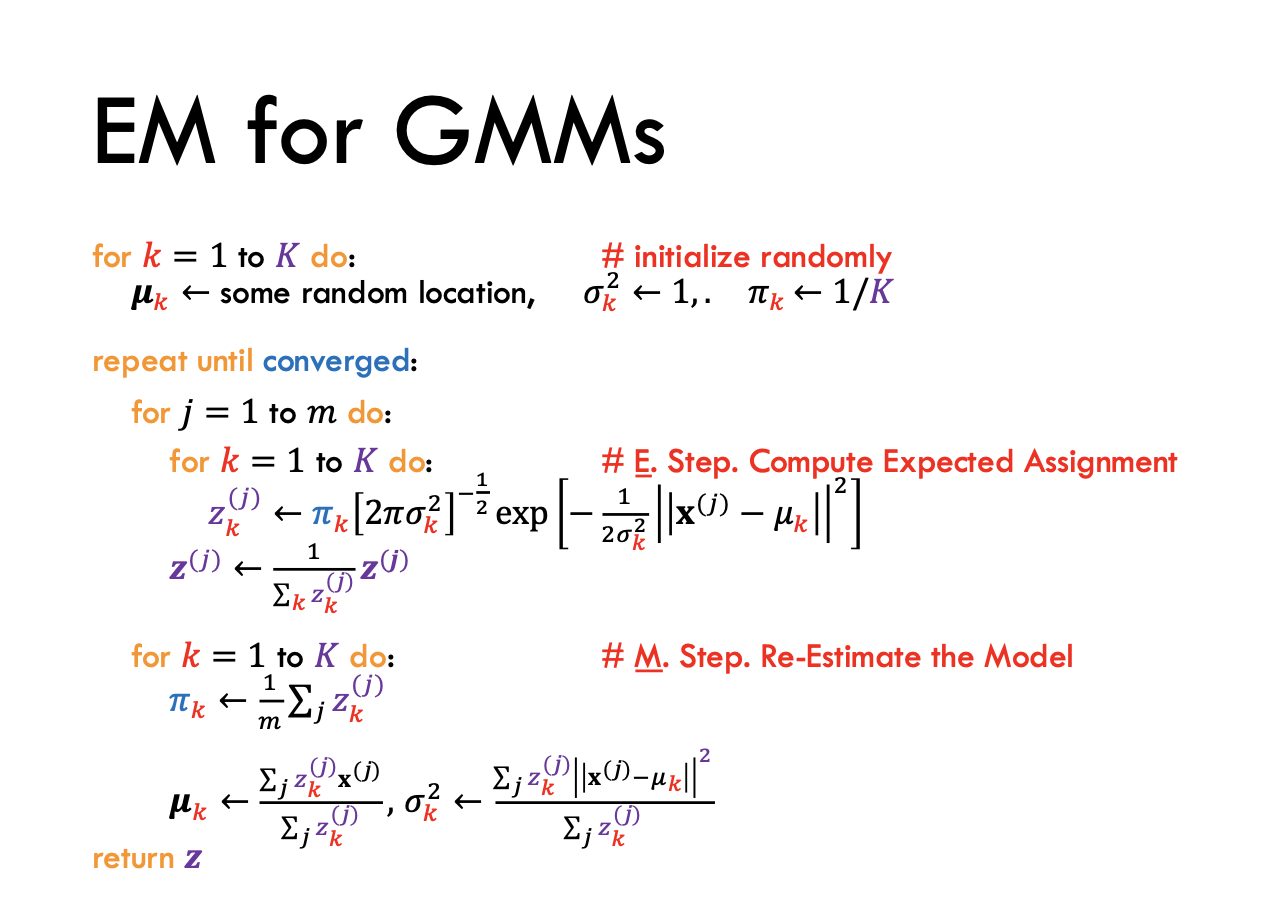
\includegraphics[height=7cm]{images/s5.png}
\subsection*{Dimensionality reduction}
May not work well for images\\
Easier means better performance

\end{document}
